% figures/counterexample_trees.tex

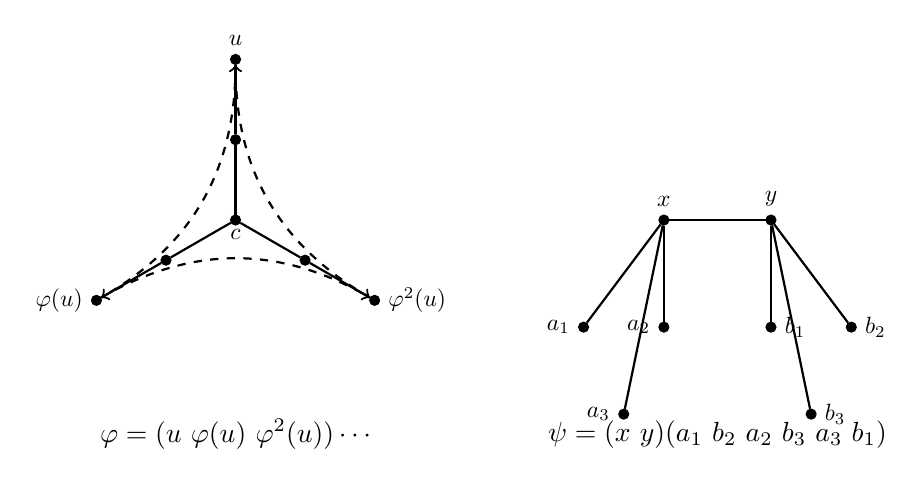
\begin{tikzpicture}[
    vertex/.style={circle, draw, fill=black, inner sep=1.5pt, minimum size=4pt},
    labeled/.style={circle, draw, fill=black, inner sep=1.5pt, minimum size=4pt, label={#1}},
    scale=0.85, every node/.style={transform shape}
]

% === Left tree: K_{1,3} with extended branches ===
\begin{scope}[shift={(-3.2,0)}]
    \node[labeled={[yshift=2pt]below:$c$}] (c) at (0,0) {};
    
    \node[vertex] (m1) at (90:1.2) {};
    \node[vertex] (m2) at (210:1.2) {};
    \node[vertex] (m3) at (330:1.2) {};
    
    \node[labeled={above:$u$}] (l1) at (90:2.4) {};
    \node[labeled={left:$\varphi(u)$}] (l2) at (210:2.4) {};
    \node[labeled={right:$\varphi^2(u)$}] (l3) at (330:2.4) {};
    
    \draw[thick] (c) -- (m1) -- (l1);
    \draw[thick] (c) -- (m2) -- (l2);
    \draw[thick] (c) -- (m3) -- (l3);
    
    \draw[->, dashed, thick, bend left=30] (l1) to (l2);
    \draw[->, dashed, thick, bend left=30] (l2) to (l3);
    \draw[->, dashed, thick, bend left=30] (l3) to (l1);
    
    \node[transform shape=false] at (0,-3.2) {$\varphi=(u\ \varphi(u)\ \varphi^2(u))\cdots$};
\end{scope}

% === Right tree: edge xy with 3 children each ===
\begin{scope}[shift={(4,0)}]
    \node[labeled={above:$x$}] (x) at (-0.8, 0) {};
    \node[labeled={above:$y$}] (y) at (0.8, 0) {};
    \draw[thick] (x) -- (y);
    
    \node[labeled={left:$a_1$}] (a1) at (-2, -1.6) {};
    \node[labeled={left:$a_2$}] (a2) at (-0.8, -1.6) {};
    \node[labeled={left:$a_3$}] (a3) at (-1.4, -2.9) {};
    
    \node[labeled={right:$b_1$}] (b1) at (0.8, -1.6) {};
    \node[labeled={right:$b_2$}] (b2) at (2, -1.6) {};
    \node[labeled={right:$b_3$}] (b3) at (1.4, -2.9) {};
    
    \draw[thick] (x) -- (a1);
    \draw[thick] (x) -- (a2);
    \draw[thick] (x) -- (a3);
    
    \draw[thick] (y) -- (b1);
    \draw[thick] (y) -- (b2);
    \draw[thick] (y) -- (b3);
    
    \node[transform shape=false] at (0,-3.2) {$\psi=(x\ y)(a_1\ b_2\ a_2\ b_3\ a_3\ b_1)$};
\end{scope}

\end{tikzpicture}